\documentclass[journal,10pt,twocolumn]{article}
\usepackage{graphicx, float}
\usepackage[margin=0.5in]{geometry}
\usepackage{amsmath, bm}
\usepackage{array}
\usepackage{booktabs}

\providecommand{\norm}[1]{\left\lVert#1\right\rVert}
\let\vec\mathbf
\newcommand{\myvec}[1]{\ensuremath{\begin{pmatrix}#1\end{pmatrix}}}
\newcommand{\mydet}[1]{\ensuremath{\begin{vmatrix}#1\end{vmatrix}}}

\title{\textbf{Circle Assignment}}
\author{Mohamed Hamdan}
\date{September 2022}

\begin{document}

\maketitle
\paragraph{\textit{Problem Statement} - Let ABC be a right triangle in which AB = 6 cm, BC = 8 cm and $\angle$B = 90°. BD is the perpendicular from B on AC. The circle through B, C, D is drawn. Construct the tangents from A to this circle.}

\section*{\large Solution}

\begin{figure}[H]
\centering
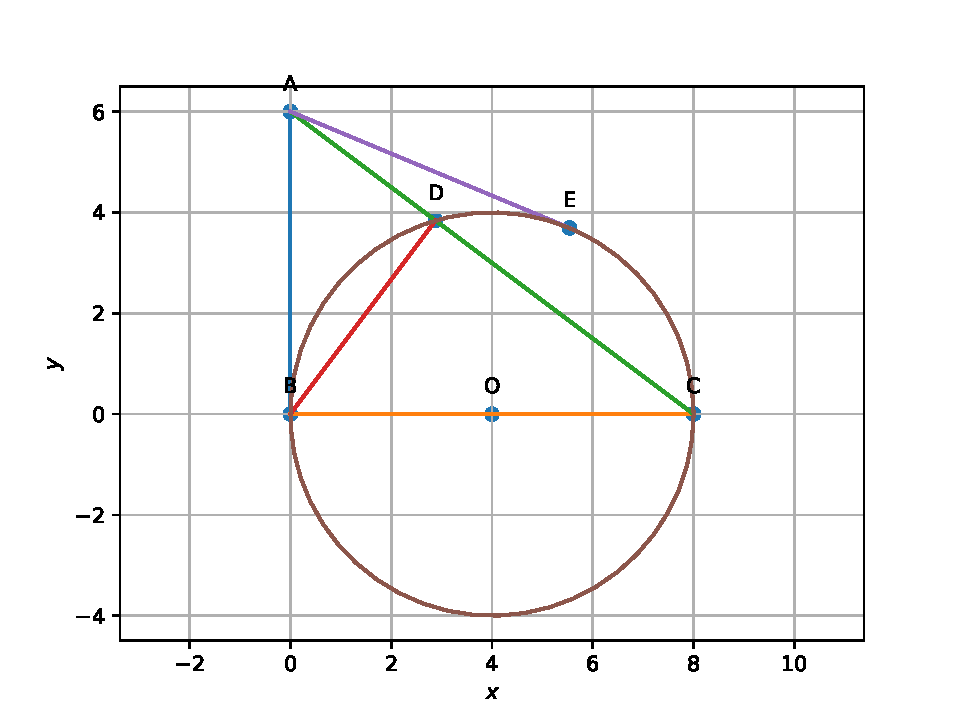
\includegraphics[width=1\columnwidth]{figs/fig1.pdf}
\caption{Tangents from A to circle through B, C and D}
\label{fig:triangle}
\end{figure}

Given that BD $\perp$ AC, which implies
\begin{equation}
\angle D = 90^\circ. 
\label{eq1}
\end{equation}

So, D can be found as the foot of the perpendicular from B on line AC. This is given by
\begin{equation}
\vec{D} = \vec{A} + \frac{\vec{m}^T(\vec{B-A})}{\norm{\vec{m}}^2}\vec{m} 
\label{eq2}
\end{equation}
where $\vec{m}$ is the direction vector for line AC.

The chord BC of the circle subtends $90^\circ$ at D. By the inclusive angle theorem, BC is the diameter of the circle with center O given by
\begin{equation}
\vec{O} = \frac{\vec{B}+\vec{C}}{2}
\label{eq3}
\end{equation}

In order to find the intersection points E and B of tangents from A, the origin is shifted from B to O. The equation of the circle in the new frame is
\begin{equation}
	\vec{x}^T\vec{x} = r^2
	\label{eq4}
\end{equation}

Let the the point of intersection between the tangent from A and the circle be P. Since P lies on the circle given by (\ref{eq4}) it is of the form    
\begin{equation}
	\vec{P} = \myvec{t \\ \sqrt{r^2-t^2}}
	\label{eq5}
\end{equation}

Since AP is a tangent to the circle, OP $\perp$ AP. This implies that
\begin{equation}
	(\vec{A}-\vec{P})^T(\vec{P}-\vec{O}) = 0
	\label{eq6}
\end{equation}

Since O is the origin in the new frame, $\vec{O} = \vec{0}$. Expanding (\ref{eq6}), we get 
\begin{equation}
	\vec{A}^T\vec{P} = \vec{P}^T\vec{P}
	\label{eq7}
\end{equation}

Substituting value of $\vec{P}$ from (\ref{eq5}) in (\ref{eq7}), we get
\begin{equation}
	\vec{A}^T\myvec{t \\ \sqrt{r^2-t^2}} = r^2	
	\label{eq8}
\end{equation}
Expanding and rearranging terms in \eqref{eq8}
\begin{multline}
	\norm{\vec{A}}^2t^2-2r^2\vec{e}_1^\top\vec{A}t+r^2(r^2-(\vec{e}_2^\top\vec{A})^2) = 0
	\label{eq:quad_t}
\end{multline}
Which is a quadratic equation in $t$ with roots given by
\begin{align}
	t = \frac{r^2\vec{e}_1^\top\vec{A}\pm\sqrt{r^4\vec{e}_1^\top\vec{A}^2-r^2\norm{\vec{A}}^2(r^2-\vec{e}_2^\top\vec{A}^2)}}{\norm{\vec{A}}^2}
	\label{eq:quad_soln}
\end{align}
Substituting the values of t from \eqref{eq:quad_soln} in \eqref{eq5} the two points of contact are obtained say $\vec{E_O}$ and $\vec{B_O}$.\\

The coordinates for position vectors $\vec{E_O}$ and $\vec{B_O}$ are with respect to origin O. The actual coordinates with respect to origin B is given by 
\begin{eqnarray}
	\vec{E} = \vec{E_O} + \vec{O}\\
	\vec{B} = \vec{B_O} + \vec{O}
\end{eqnarray}

\section*{\large Construction}
The input parameters are the lengths
\begin{eqnarray*}
	AB = a = 6\\
	BC = b = 8
\end{eqnarray*}
{
\setlength\extrarowheight{5pt}
\begin{tabular}{|c|c|c|}
	\hline
	\textbf{Symbol}&\textbf{Value}&\textbf{Description}\\
	\hline
	a&6&AB\\
	\hline
	b&8&BC\\
	\hline
	r&$\frac{b}{2}$&Radius\\
	\hline
	$\vec{m}$&$\vec{A-C}$&Direction vector of line AC\\
	\hline
	$\vec{D}$&$\vec{A} + \frac{\vec{m}^T(\vec{B-A})}{\norm{\vec{m}}^2}\vec{m}$&Point D\\[5pt]
	\hline
	$\vec{A_O}$&$\vec{A-O}$&$\vec{A}$ when origin shifted to $\vec{O}$\\
	\hline
	$t_1,t_2$&evaluate \eqref{eq:quad_soln}&solution of \eqref{eq:quad_t}\\[5pt] 
	\hline
	$\vec{E}$&$\myvec{t_1 \\ \sqrt{r^2-t_1^2}}+\vec{O}$&Point E\\[5pt]
	\hline
	$\vec{B}$&$\myvec{t_2 \\ \sqrt{r^2-t_2^2}}+\vec{O}$&Point B\\[5pt]
	\hline
\end{tabular}
}

\section*{\large Proofs}
\subsection*{\normalsize Foot of perpendicular from point $\vec{P}$ on line $\vec{A}+\lambda\vec{m}$}
Let the intersection point be $\vec{X}$. Since X is foot of perpendicular from point P to line with direction vector $\vec{m}$,
\begin{equation}
	\vec{m}^T(\vec{X-P}) = 0
	\label{pf1-eq-1}
\end{equation}
Since X lies on the line with direction vector $\vec{m}$,
\begin{equation}
	\vec{X} = \vec{A}+\lambda\vec{m}
	\label{pf1-eq-2}
\end{equation}
Substituting (\ref{pf1-eq-2}) in (\ref{pf1-eq-1}) and solving for $\lambda$,
\begin{equation}
	\lambda = \frac{\vec{m}^T(\vec{P-A})}{\norm{\vec{m}}^2}
	\label{pf1-eq-3}
\end{equation}
Substituting (\ref{pf1-eq-3}) in (\ref{pf1-eq-2}),
\begin{equation}
\vec{X} = \vec{A} + \frac{\vec{m}^T(\vec{P-A})}{\norm{\vec{m}}^2}\vec{m} 
\end{equation}

\subsection*{\normalsize Inclusive angle theorem}
The inclusive angle theorem states that the angle subtended by any chord at the center of a circle is twice the angle angle subtended by the same chord at any other point on the major segment. Take three points A, B, and C on a unit circle at angles $\theta$, $\phi$ and $\psi$. Then,
\begin{eqnarray}
	\vec{A} = \myvec{cos\theta\\sin\theta},
	\vec{B} = \myvec{cos\phi\\sin\phi},
	\vec{C} = \myvec{cos\psi\\sin\psi}
\end{eqnarray}

Let AB be the chord that subtends angles at the center O and at point C. The cosine of the angle subtended at point C is given by
\begin{align}
	cos(\angle ACB) = \frac{\langle A-C, B-C\rangle}{|A-C||B-C|}
	\label{pf2-eq-1}
\end{align}

Where
\begin{multline*}
	\langle A-C, B-C\rangle = \langle (\cos\theta-\cos\psi,\sin\theta-\sin\psi),(\cos\phi-\cos\psi,\\
	\sin\phi-\sin\psi)\rangle
	\end{multline*}
\begin{multline*}
	= (\cos\theta-\cos\psi)(\cos\phi-\cos\psi)+(\sin\theta-\sin\psi)\\
	(\sin\phi-\sin\psi)
\end{multline*}
\begin{multline*}
	= -2\sin\frac{\theta-\psi}2\sin\frac{\theta+\psi}2 \cdot(-2)\sin\frac{\phi-\psi}2\sin\frac{\phi+\psi}2 \\\quad+ 2\cos\frac{\theta+\psi}2\sin\frac{\theta-\psi}2 \cdot 2\cos\frac{\phi+\psi}2\sin\frac{\phi-\psi}2
\end{multline*}
\begin{multline*}
	= 4\sin\frac{\theta-\psi}2\sin\frac{\phi-\psi}2(\sin\frac{\theta+\psi}2\sin\frac{\phi+\psi}2+\\
	\cos\frac{\theta+\psi}2\cos\frac{\phi+\psi}2)
\end{multline*}
\begin{align*}
	= 4\sin\frac{\theta-\psi}2\sin\frac{\phi-\psi}2\cos\left(\frac{\theta+\psi}2-\frac{\phi+\psi}2\right)
\end{align*}
\begin{align}
	= 4\sin\frac{\theta-\psi}2\sin\frac{\phi-\psi}2\cos\frac{\theta-\phi}2
	\label{pf2-eq-2}
\end{align}

\begin{multline*}
	|A-C|^2|B-C|^2 = ((\cos\theta-\cos\psi)^2+(\sin\theta-\sin\psi)^2)\\
	((\cos\phi-\cos\psi)^2+(\sin\phi-\sin\psi)^2)
\end{multline*}
\begin{multline*}
	= (2-2\cos\theta\cos\psi - 2\sin\theta\sin\psi)(2-\\
	2\cos\phi\cos\psi - 2\sin\phi\sin\psi)
\end{multline*}
\begin{align*}
	&= 4(1-\cos(\theta-\psi))(1-\cos(\phi-\psi))\\
	&= 4\cdot 2\sin^2\frac{\theta-\psi}2\cdot 2\sin^2\frac{\phi-\psi}2
\end{align*}
\begin{align}
	&= 16 \sin^2\frac{\theta-\psi}2\sin^2\frac{\phi-\psi}2
	\label{pf2-eq-3}
\end{align}

Substituting (\ref{pf2-eq-2}) and (\ref{pf2-eq-3}) in (\ref{pf2-eq-1}),
\begin{equation}
	cos(\angle ACB) = cos(\frac{\theta-\phi}{2})	
\end{equation}
Hence $\angle ACB = \frac{\theta-\phi}{2} = \frac{\angle AOB}{2}$

\end{document}
